% ドキュメントの設定
\documentclass[a4paper,11pt,xelatex,ja=standard]{bxjsarticle}
\usepackage{tikz}
\usetikzlibrary {datavisualization.formats.functions}
\usepackage{pgfplots}
\usepackage{float}
\usepackage{amsmath}

% ドキュメント開始
\begin{document}

\section{実験の目的}
    ネットワークアナライザを用いたアンテナのインピーダンス測定,2ポート測定法,Sパラメータ,ワイヤレス電力伝送効率の求め方を学び電磁界解析の結果と比較できる.

\section{実験の理論または原理}
    特性インピーダンス𝑍0が50 [Ω]のときの,反射係数は,(1)式で表される.
    \[\Gamma = \frac{𝑍𝐿−𝑍0}{𝑍𝐿+𝑍0} = \frac{𝑍𝐿−50}{𝑍𝐿+50} \tag{1}\]
    ここで𝑍𝐿は負荷インピーダンスである.
    スミスチャートは,この反射係数を複素平面で表したものと,考えることができる.
    VSWR(定在波比)は(2)式で表される.
    \[\text{VSWR} = \frac{1+|\Gamma|}{1−|\Gamma|} \tag{2}\]
    リターンロスReturn Loss RLは
    \[𝑅𝐿 = 20\log_{10}|\Gamma| \tag{3}\]
    これはSパラメータの𝑆_{11}と同じである
    散乱行列(Sパラメータ)
    \[𝑆 = \begin{bmatrix}𝑆_{11} & 𝑆_{12} \\𝑆_{21} & 𝑆_{22}\end{bmatrix}\]
    透過係数は𝑆_{21}と同じである.
    スミスチャート上で,反射係数の絶対値が,0.5以下となる範囲はどこか考えてみましょう
    \[\Gamma = \frac{𝑍𝐿− 𝑍0}{𝑍𝐿 + 𝑍0} = \frac{𝑍𝐿− 50}{𝑍𝐿 + 50} = 0.5\]

\section{実験の結果}
    \subsection{各種コネクタのインピーダンス測定}
        各種コネクタのインピーダンス測定において、まず校正が正しく行われていることを確認するために、事前に値が分かっている校正用コネクタを負荷として接続し、測定を行いました。Open、Short、Loadの各ケースについて実施し、事前課題の理論値と比較しました。特に、OpenとShortについてはそれぞれの測定が正常に行われ、理論値と比較して許容範囲内の結果を得ることができました。

        若干の誤差は変換コネクタによって位相がずれていることである。

        \begin{figure}[H]
            \centering
            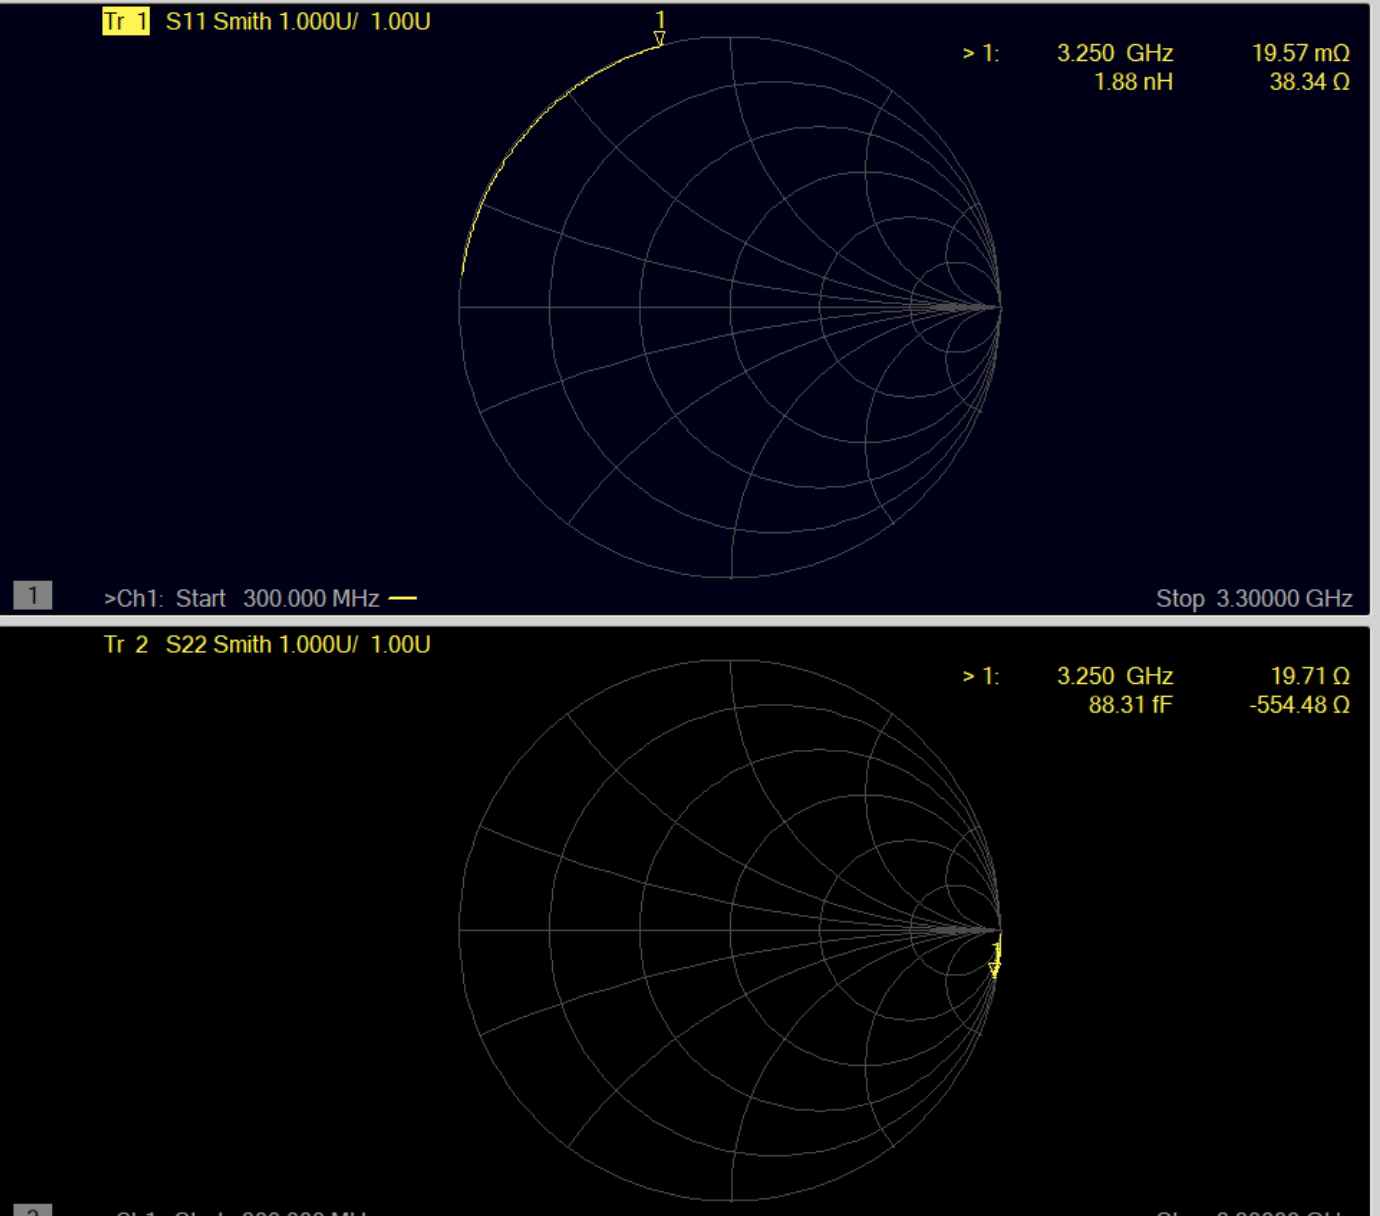
\includegraphics[width=0.5\textwidth]{./img/24-3/1.png}
            \caption{Openとshort}
        \end{figure}

        \begin{figure}[H]
            \centering
            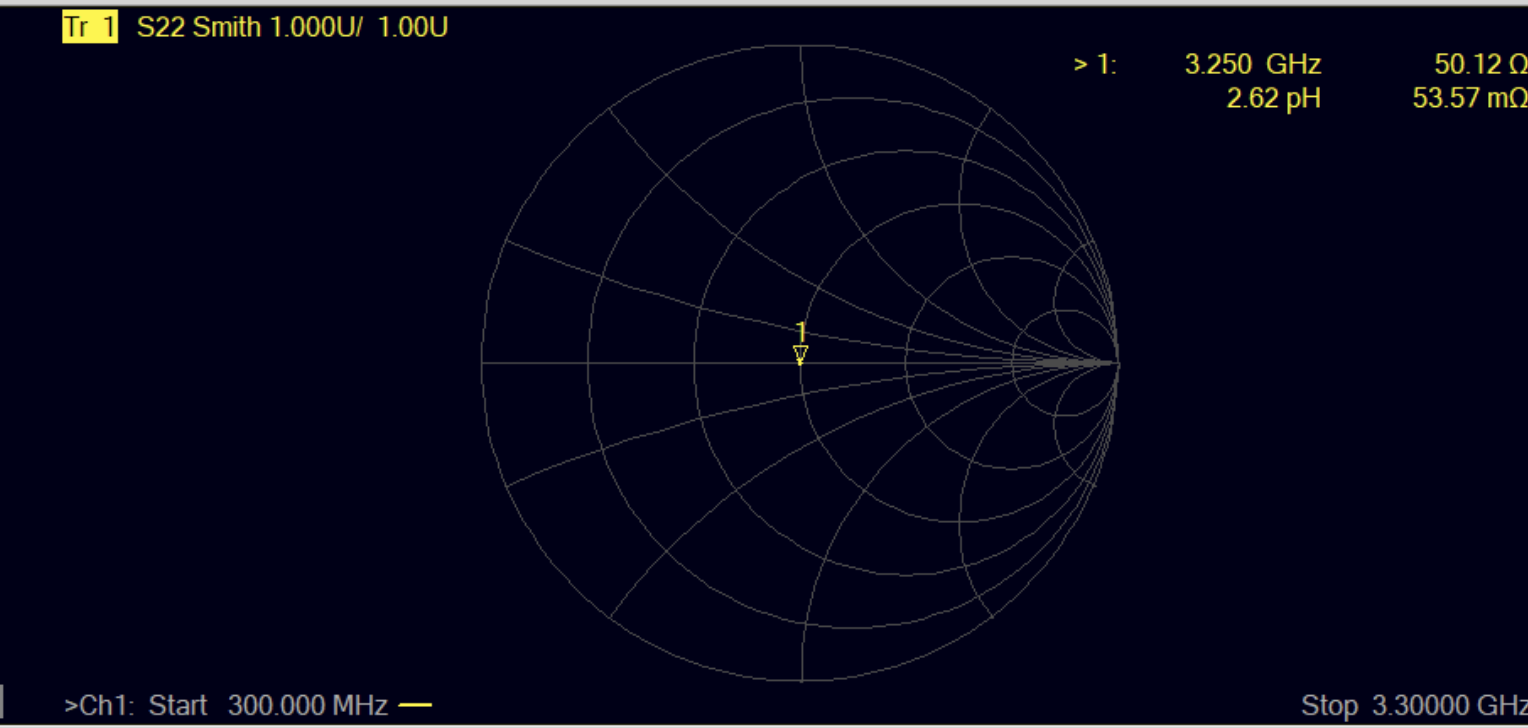
\includegraphics[width=0.5\textwidth]{./img/24-3/2.png}
            \caption{load}
        \end{figure}

    \subsection{ダイポールアンテナの測定}
        ダイポールアンテナのインピーダンス測定を実施しました。
        
        \begin{table}[H]
            \centering
            \begin{tabular}{|c|c|c|}
                \hline
                No & 内容 & 値 \\
                \hline
                3 & アンテナの形状の特徴 &  ダイポール\\
                \hline
                4 & アンテナの太さの直径 [mm] &  5\\
                \hline
                5 & アンテナの長さ [mm] &  255\\
                \hline
            \end{tabular}
            \caption{測定アンテナの仕様}
        \end{table}

        表に示した仕様に基づいて、アンテナのインピーダンスを測定しました。測定結果は図1に示すように、OpenとShortの状態でのインピーダンス特性を確認しました。

        \begin{figure}[H]
            \centering
            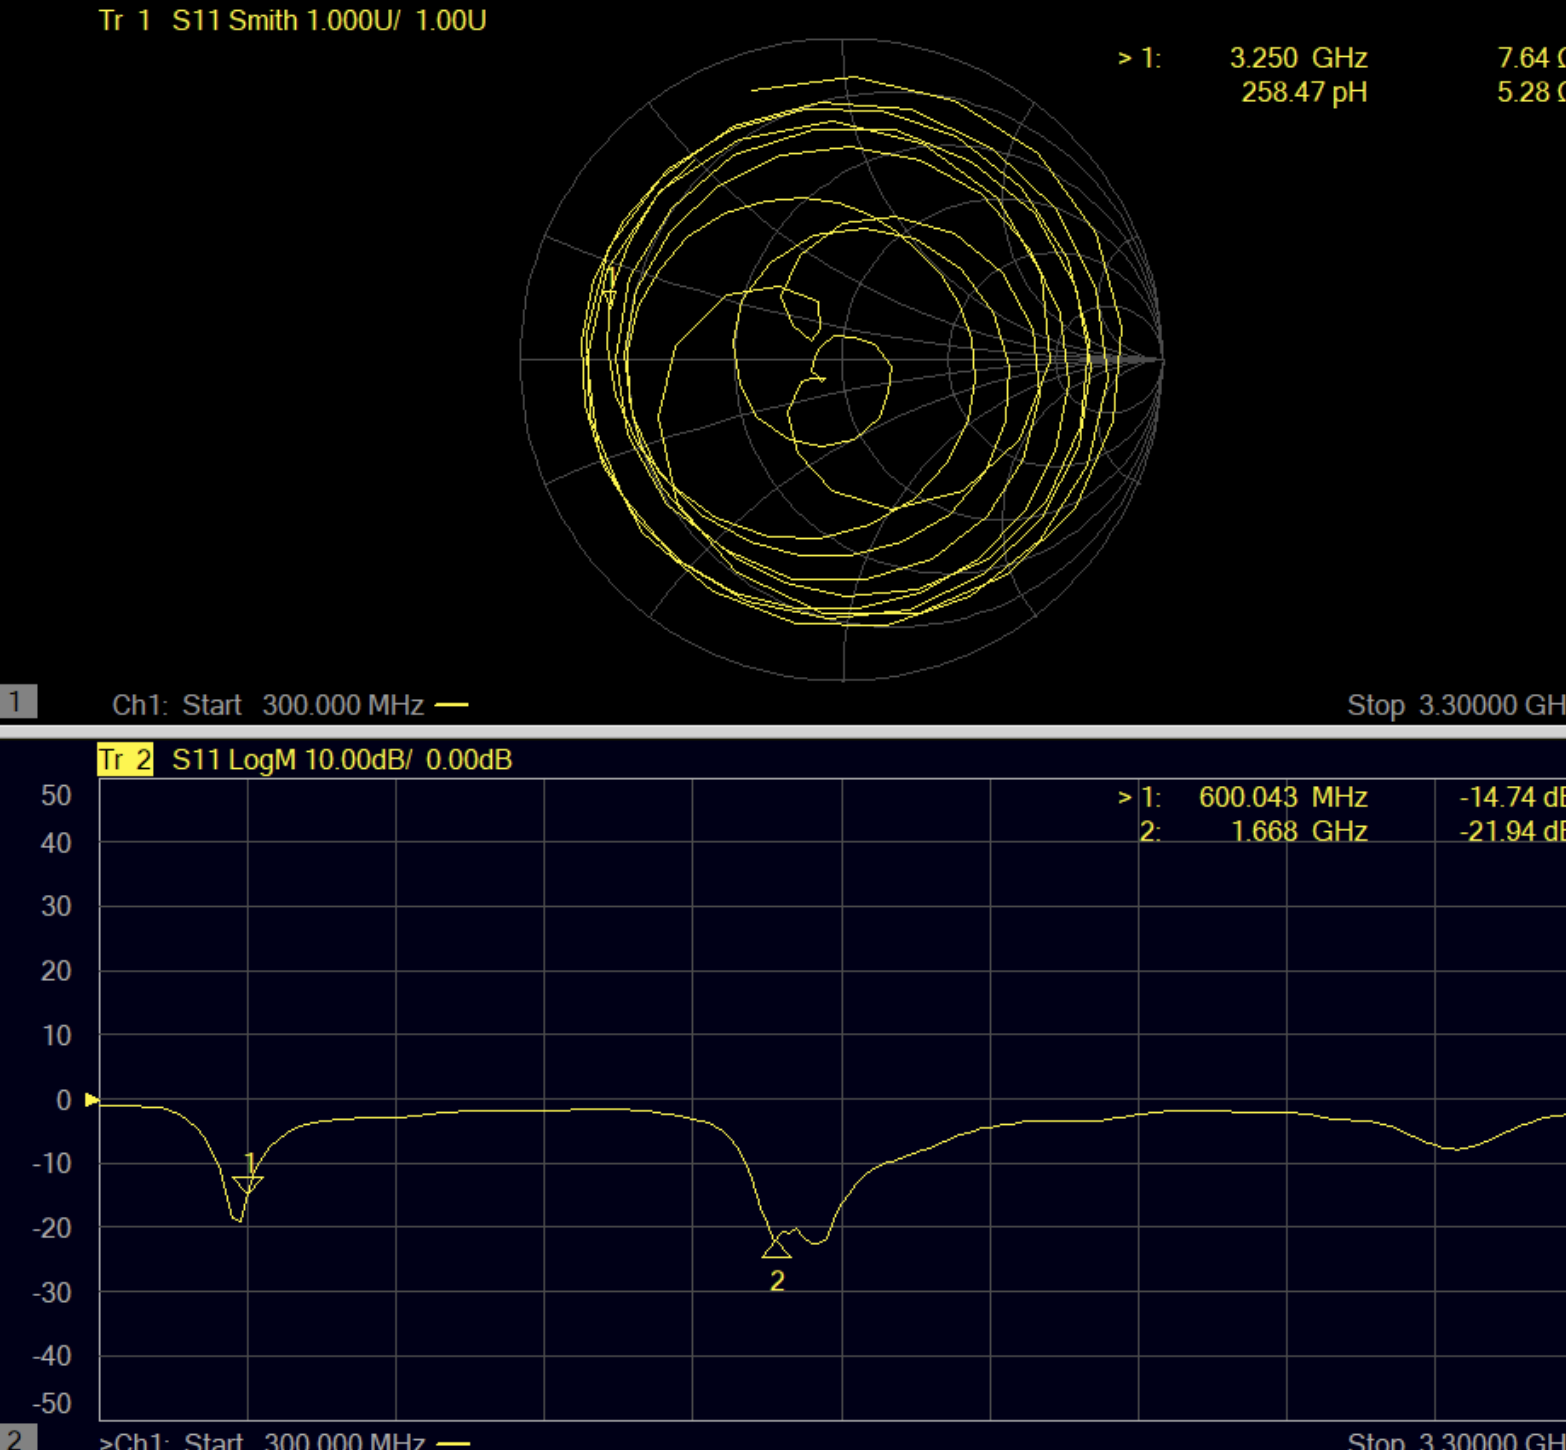
\includegraphics[width=0.5\textwidth]{./img/24-3/3.png}
            \caption{Openとshort}
        \end{figure}

    \subsection{2ポート測定}
        \subsubsection{アンテナ作成}
            600 MHzで共振するアンテナを2台セミリジッドケーブルと, 銅線を用いて作成する.
        \subsubsection{Sパラメータの測定}
            二つのアンテナ間の距離を125mm としてSパラメータを測定する
            \begin{figure}[H]
                \centering
                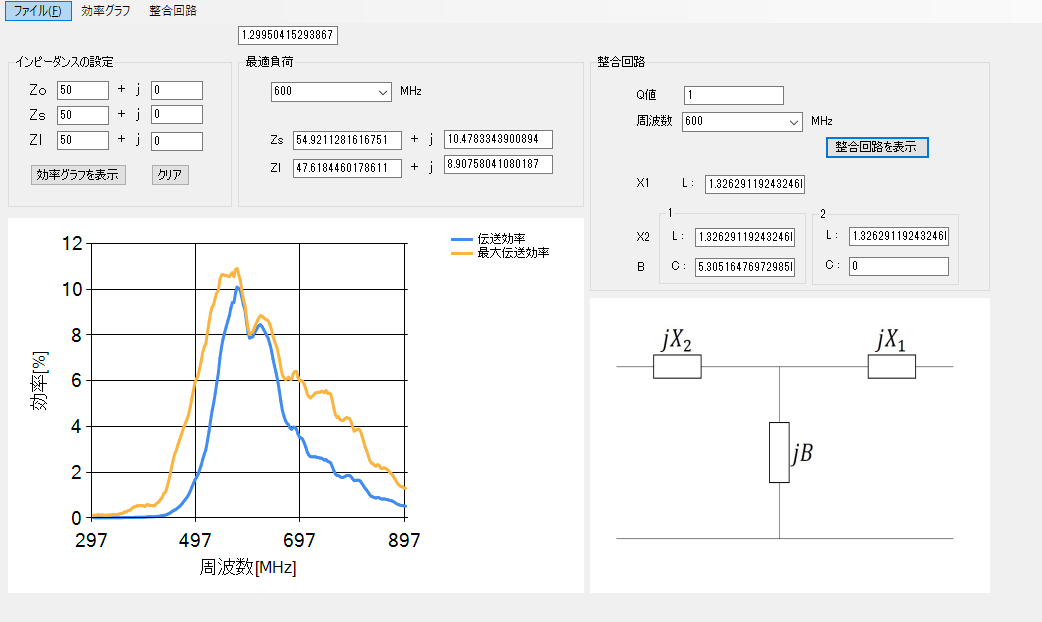
\includegraphics[width=0.5\textwidth]{./img/24-3/4.png}
                \caption{load}
            \end{figure}


\section{参考文献}

\end{document}